\documentclass[12pt,letterpaper,noanswers]{exam}
\usepackage[usenames,dvipsnames,svgnames,table]{xcolor}
\usepackage[margin=0.9in]{geometry}
\renewcommand{\familydefault}{\sfdefault}
\usepackage{multicol}
\pagestyle{head}
\header{AM 111 Class 18}{}{Numerical differentiation, p.\thepage}
\runningheadrule
\headrule
\usepackage{siunitx}
\usepackage{graphicx} % more modern
\usepackage{amsmath} 
\usepackage{amssymb} 
\usepackage{hyperref}
\usepackage{tcolorbox}
\usepackage{enumitem}
\def\mbf{\mathbf}
\newcommand{\vc}[1]{\boldsymbol{#1}}
\def\dsst{\displaystyle}
\DeclareMathOperator*{\argmin}{arg\,min} % thin space, limits underneath in displays


\begin{document}
 \pdfpageheight 11in 
  \pdfpagewidth 8.5in

\noindent 

\section*{Preliminaries}

\begin{itemize}
\itemsep0pt
\item The problem set and project proposal are due tomorrow.
\item The skill check below is for the following class.
\end{itemize}


\noindent\textbf{Big picture}

Today: Approximating $\frac{df}{dx}$ at a point $x_0$.

\vspace{0.2cm}
\hrule
\vspace{0.2cm}

\noindent \textbf{Skill check practice}

Identify the order of the method if 
\[f''(x) \approx \dfrac{f(x-h)-2f(x)+f(x+h)}{h^2}\]
is used to approximate the second derivative.

\noindent Extra info: Using Taylor expansion, it is possible to show that \[f''(x) = \dfrac{f(x-h)-2f(x)+f(x+h)}{h^2} - \frac{1}{12}h^2 f^{(4)}(x) + \mathcal{O}(h^4).\]

\emph{You do not need to derive this yourself.}


\vspace{0.2cm}
\hrule
\vspace{0.2cm}

\noindent \textbf{Skill check solution}
Answer: second order method

Explanation: The order of the method comes from the exponent of $h$ in the first error term.  That term is $\frac{1}{12}h^2f''''(x)$, so the exponent is $2$, and this is a second order method.

\vspace{0.2cm}
\hrule
\vspace{0.2cm}


\section*{Numerical differentiation}


\subsection*{Approximating a derivative from data}

\begin{enumerate}[resume=classQ]
\item Assume the maximum measurement error is $\delta \vert f(x_i)\vert$.  Replace $\epsilon_{\text{mach}}$ in your rounding error calculation for forward and central differences with $\delta \vert f(x_i)\vert$ to find expressions for the maximum error due to measurement error.

\vspace{1in}


%then it propagates to the derivative as $\dfrac{\delta}{h}(\vert f(x_{i+1})\vert + \vert f(x_{i})\vert)$ where $h = x_{i+1}-x_i$.
\end{enumerate}


\begin{enumerate}[resume=classQ]
\item Consider the three functions plotted on the left below.  
\begin{parts}
\item What is the largest difference in $y$ that occurs between any two functions?  What is the smallest difference?
\vspace{1cm}
\item Find the derivative of each function.
\vspace{1in}
\item If the true function were $f(x) = x$, but your measurement method added high frequency noise, so that the data looked exactly like $x + 0.01\sin(100x)$, what is the maximum error you would see in the derivative?
\vspace{1cm}

%\item Thinking of your derivative as your output (where error in the output is forward error) and your measurements as your input (with error ibackward error), create an estimate of an absolute condition number.
\vspace{1cm}
\end{parts}



\end{enumerate}

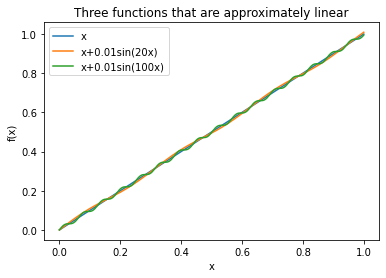
\includegraphics[width = 0.45\linewidth]{img/Class11lines.png}
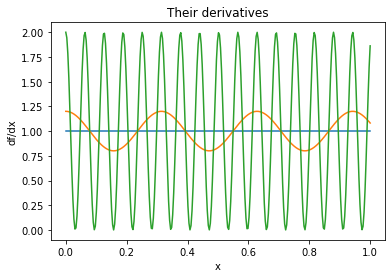
\includegraphics[width = 0.45\linewidth]{img/Class11linederiv.png}

% \begin{enumerate}[resume=classQ]
% \item 
% \end{enumerate}



\subsection*{Richardson extrapolation}

\begin{tcolorbox}

(Greenbaum and Chartier \S 9.2)

Central differences: $f'(x) = \dfrac{f(x+h)-f(x-h)}{2h} - \dfrac{1}{6}h^2 f'''(x) + \mathcal{O}(h^4)$

Let $\phi_0(h) = \dfrac{f(x+h)-f(x-h)}{2h}$, so that $f'(x) = \phi_0(h) - \dfrac{1}{6}h^2 f'''(x) + \mathcal{O}(h^4)$
\end{tcolorbox}
\begin{enumerate}[resume=classQ]
\item We have $f'(x) = \phi_0(h) + \frac{1}{6}h^2 f'''(x) + \mathcal{O}(h^4)$.

Similarly, $f'(x) = \phi_0(h/2) + \frac{1}{6}(h/2)^2 f'''(x) +  \mathcal{O}(h^4)$.

Multiply the second equation by $4$ and subtract the first equation to cancel the $h^2$ terms.  Then rearrange to find a formula of the form $f'(x) = a\phi_0(h/2) + b\phi_0(h) + \mathcal{O}(h^4)$.

What order is this method?
\vspace{1in}

\item The forward difference formula can be written $f'(x) = \dfrac{f(x+h)-f(x)}{h} + \frac{1}{2} hf''(x) + \mathcal{O}(h^2)$.  In this case let $\phi_0(h) = \dfrac{f(x+h)-f(x)}{h}$.  Find an analogous formula to the one above.

What order is this method?

\vspace{1in}

\item The plots below show the error with and without using Richardson extrapolation for forward differences (left) and for central differences (right).
\begin{parts}
\item Does Richardson extrapolation impact the way the rounding error depends on $h$?
\vspace{0.5cm}

\item Check the slope of the truncation error on the log-log plot.  Does this match the expected order from above?
\end{parts}
\end{enumerate}

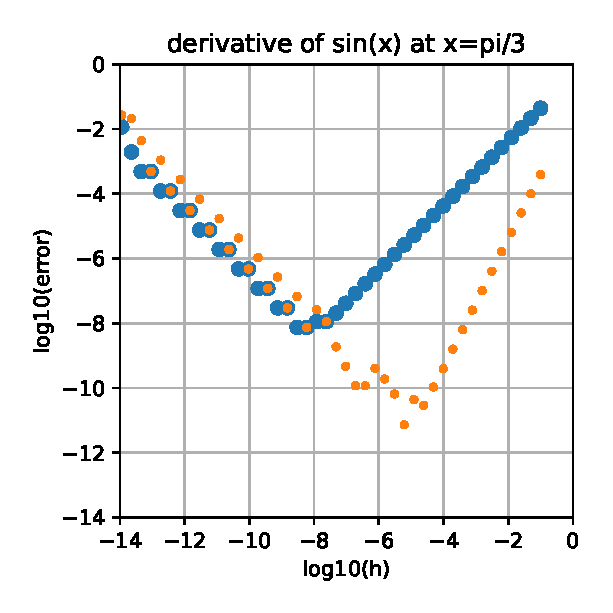
\includegraphics[width=0.5\linewidth]{img/Class12sinforwardR.eps}
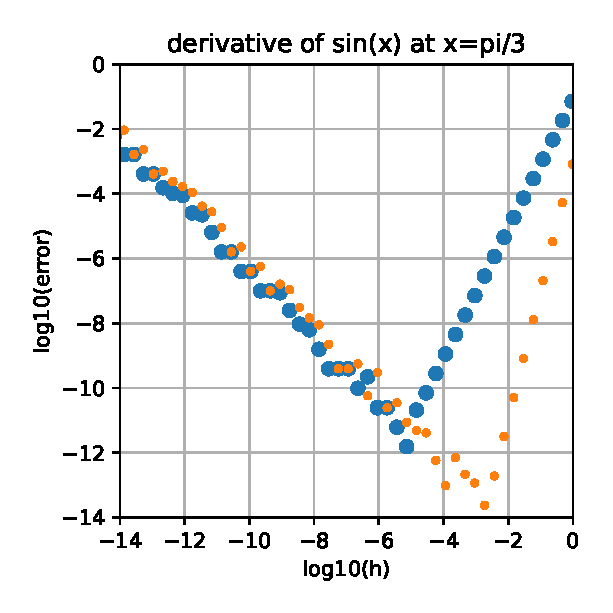
\includegraphics[width=0.5\linewidth]{img/Class12sincentralR.eps}

\subsubsection*{Implementation}
\begin{enumerate}[resume=classQ]
\item Let \texttt{hvals} be an array of $h$ values (of length $N$) and \texttt{deriv} be the true value of $\frac{d}{dx}\sin x$ at $x = \pi/3$.
\begin{parts}
\item Write code for finding \texttt{error[k]}, the error associated with estimating $f'(x)$ (without using extrapolation) for $h =$\texttt{hvals[k]}.
\vspace{1in}

\item Write code for finding \texttt{extrapError[k]}, the error associated with estimating $f'(x)$ using extrapolation.  %It is your choice whether $h =$\texttt{hlist[k]} or $h/2 =$\texttt{hlist[k]}
\vspace{1in}

\item Write code for a loop that generates $N$ values of \texttt{error}.
\vspace{1.5in}

\item Vectorize your code.

Example:
\begin{verbatim}
# preliminaries
import numpy as np
f = np.sin
x0 = np.pi/3
h0 = 0.1
N = 52
\end{verbatim}

\begin{verbatim}
# using a loop
hvals = np.zeros(N)
yvals = np.zeros(N)
for k in range(N):
    hvals[k] = h0
    yvals[k] = f(x0+h0)
    h0 = h0/2
\end{verbatim}


\begin{verbatim}
# switching to vectorized
hvals = np.array([h0*2**(-k) for k in range(N)])
yvals = f(hvals+x0)
\end{verbatim}



% Add to your pseudocode in order to generate $N$ values of \texttt{extrapError}.  
\vspace{1in}
\end{parts}
\end{enumerate}


% \eject
% \section*{Some Review Qs from Heath}
% \S 1 Review (T/F)
% \begin{enumerate}
%     \item[1.1] A problem is ill-conditioned if its solution is highly sensitive to small changes in the problem data.
%     \item[1.3] The conditioning of a problem depends on the algorithm used to solve it.
%     \item[1.10] In a floating point number system, the underflow level is the smallest positive number that perturbs the number $1$ when added to it.
% \end{enumerate}

% \noindent \S 3 Review
% \begin{enumerate}
%     \item[3.13] In an overdetermined linear least squares problem with model function $f(x,\vc{w}) = w_1\phi_1(x) + w_2\phi_2(x) + w_3\phi_3(x)$, what will be the rank of the resulting least squares matrix $A$ if we take $\phi_1(x) = 1$, $\phi_2(x) = x$, and $\phi_3(x) = 1-x$.
%     \item[3.14] What is the system of normal equations for the linear least squares problem $A\vc{w}\cong\vc{y}$?
% \end{enumerate}

% \noindent \S 5 Review
% \begin{enumerate}
%     \item[5.3] (T/F) If an iterative method for solving a nonlinear equation gains more than one bit of accuracy per iteration, then it is said to have a superlinear convergence rate.
%     \item[5.6] What is meant by a \emph{bracket} for a nonlinear function in one dimension?  What does this concept have to do with zero-finding? 
%     \item[5.10] What condition ensures that the bisection method will find a zero of a continuous nonlinear function $f$ in the interval $[a,b]$?
% \end{enumerate}

% \noindent \S 7 Review
% \begin{enumerate}
%     \item[7.1] (T/F) There are arbitrarily many different mathematical functions that interpolate a given set of data points.
%     \item[7.4] (T/F) When interpolating a continuous function by a polynomial at equally spaced points on a given interval, the polynomial interpolant always converges to the function as the number of interpolation points increases.
%     \item[7.5] What is the basic distinction between interpolation and approximation of a function?
% \end{enumerate}
\end{document}